\documentclass[]{book}
\usepackage{lmodern}
\usepackage{amssymb,amsmath}
\usepackage{ifxetex,ifluatex}
\usepackage{fixltx2e} % provides \textsubscript
\ifnum 0\ifxetex 1\fi\ifluatex 1\fi=0 % if pdftex
  \usepackage[T1]{fontenc}
  \usepackage[utf8]{inputenc}
\else % if luatex or xelatex
  \ifxetex
    \usepackage{mathspec}
  \else
    \usepackage{fontspec}
  \fi
  \defaultfontfeatures{Ligatures=TeX,Scale=MatchLowercase}
\fi
% use upquote if available, for straight quotes in verbatim environments
\IfFileExists{upquote.sty}{\usepackage{upquote}}{}
% use microtype if available
\IfFileExists{microtype.sty}{%
\usepackage{microtype}
\UseMicrotypeSet[protrusion]{basicmath} % disable protrusion for tt fonts
}{}
\usepackage{hyperref}
\hypersetup{unicode=true,
            pdftitle={A Minimal Book Example},
            pdfauthor={Yihui Xie},
            pdfborder={0 0 0},
            breaklinks=true}
\urlstyle{same}  % don't use monospace font for urls
\usepackage{natbib}
\bibliographystyle{apalike}
\usepackage{color}
\usepackage{fancyvrb}
\newcommand{\VerbBar}{|}
\newcommand{\VERB}{\Verb[commandchars=\\\{\}]}
\DefineVerbatimEnvironment{Highlighting}{Verbatim}{commandchars=\\\{\}}
% Add ',fontsize=\small' for more characters per line
\usepackage{framed}
\definecolor{shadecolor}{RGB}{248,248,248}
\newenvironment{Shaded}{\begin{snugshade}}{\end{snugshade}}
\newcommand{\KeywordTok}[1]{\textcolor[rgb]{0.13,0.29,0.53}{\textbf{#1}}}
\newcommand{\DataTypeTok}[1]{\textcolor[rgb]{0.13,0.29,0.53}{#1}}
\newcommand{\DecValTok}[1]{\textcolor[rgb]{0.00,0.00,0.81}{#1}}
\newcommand{\BaseNTok}[1]{\textcolor[rgb]{0.00,0.00,0.81}{#1}}
\newcommand{\FloatTok}[1]{\textcolor[rgb]{0.00,0.00,0.81}{#1}}
\newcommand{\ConstantTok}[1]{\textcolor[rgb]{0.00,0.00,0.00}{#1}}
\newcommand{\CharTok}[1]{\textcolor[rgb]{0.31,0.60,0.02}{#1}}
\newcommand{\SpecialCharTok}[1]{\textcolor[rgb]{0.00,0.00,0.00}{#1}}
\newcommand{\StringTok}[1]{\textcolor[rgb]{0.31,0.60,0.02}{#1}}
\newcommand{\VerbatimStringTok}[1]{\textcolor[rgb]{0.31,0.60,0.02}{#1}}
\newcommand{\SpecialStringTok}[1]{\textcolor[rgb]{0.31,0.60,0.02}{#1}}
\newcommand{\ImportTok}[1]{#1}
\newcommand{\CommentTok}[1]{\textcolor[rgb]{0.56,0.35,0.01}{\textit{#1}}}
\newcommand{\DocumentationTok}[1]{\textcolor[rgb]{0.56,0.35,0.01}{\textbf{\textit{#1}}}}
\newcommand{\AnnotationTok}[1]{\textcolor[rgb]{0.56,0.35,0.01}{\textbf{\textit{#1}}}}
\newcommand{\CommentVarTok}[1]{\textcolor[rgb]{0.56,0.35,0.01}{\textbf{\textit{#1}}}}
\newcommand{\OtherTok}[1]{\textcolor[rgb]{0.56,0.35,0.01}{#1}}
\newcommand{\FunctionTok}[1]{\textcolor[rgb]{0.00,0.00,0.00}{#1}}
\newcommand{\VariableTok}[1]{\textcolor[rgb]{0.00,0.00,0.00}{#1}}
\newcommand{\ControlFlowTok}[1]{\textcolor[rgb]{0.13,0.29,0.53}{\textbf{#1}}}
\newcommand{\OperatorTok}[1]{\textcolor[rgb]{0.81,0.36,0.00}{\textbf{#1}}}
\newcommand{\BuiltInTok}[1]{#1}
\newcommand{\ExtensionTok}[1]{#1}
\newcommand{\PreprocessorTok}[1]{\textcolor[rgb]{0.56,0.35,0.01}{\textit{#1}}}
\newcommand{\AttributeTok}[1]{\textcolor[rgb]{0.77,0.63,0.00}{#1}}
\newcommand{\RegionMarkerTok}[1]{#1}
\newcommand{\InformationTok}[1]{\textcolor[rgb]{0.56,0.35,0.01}{\textbf{\textit{#1}}}}
\newcommand{\WarningTok}[1]{\textcolor[rgb]{0.56,0.35,0.01}{\textbf{\textit{#1}}}}
\newcommand{\AlertTok}[1]{\textcolor[rgb]{0.94,0.16,0.16}{#1}}
\newcommand{\ErrorTok}[1]{\textcolor[rgb]{0.64,0.00,0.00}{\textbf{#1}}}
\newcommand{\NormalTok}[1]{#1}
\usepackage{longtable,booktabs}
\usepackage{graphicx,grffile}
\makeatletter
\def\maxwidth{\ifdim\Gin@nat@width>\linewidth\linewidth\else\Gin@nat@width\fi}
\def\maxheight{\ifdim\Gin@nat@height>\textheight\textheight\else\Gin@nat@height\fi}
\makeatother
% Scale images if necessary, so that they will not overflow the page
% margins by default, and it is still possible to overwrite the defaults
% using explicit options in \includegraphics[width, height, ...]{}
\setkeys{Gin}{width=\maxwidth,height=\maxheight,keepaspectratio}
\IfFileExists{parskip.sty}{%
\usepackage{parskip}
}{% else
\setlength{\parindent}{0pt}
\setlength{\parskip}{6pt plus 2pt minus 1pt}
}
\setlength{\emergencystretch}{3em}  % prevent overfull lines
\providecommand{\tightlist}{%
  \setlength{\itemsep}{0pt}\setlength{\parskip}{0pt}}
\setcounter{secnumdepth}{5}
% Redefines (sub)paragraphs to behave more like sections
\ifx\paragraph\undefined\else
\let\oldparagraph\paragraph
\renewcommand{\paragraph}[1]{\oldparagraph{#1}\mbox{}}
\fi
\ifx\subparagraph\undefined\else
\let\oldsubparagraph\subparagraph
\renewcommand{\subparagraph}[1]{\oldsubparagraph{#1}\mbox{}}
\fi

%%% Use protect on footnotes to avoid problems with footnotes in titles
\let\rmarkdownfootnote\footnote%
\def\footnote{\protect\rmarkdownfootnote}

%%% Change title format to be more compact
\usepackage{titling}

% Create subtitle command for use in maketitle
\providecommand{\subtitle}[1]{
  \posttitle{
    \begin{center}\large#1\end{center}
    }
}

\setlength{\droptitle}{-2em}

  \title{A Minimal Book Example}
    \pretitle{\vspace{\droptitle}\centering\huge}
  \posttitle{\par}
    \author{Yihui Xie}
    \preauthor{\centering\large\emph}
  \postauthor{\par}
      \predate{\centering\large\emph}
  \postdate{\par}
    \date{2020-01-15}

\usepackage{booktabs}

\begin{document}
\maketitle

{
\setcounter{tocdepth}{1}
\tableofcontents
}
\chapter{Prerequisites}\label{prerequisites}

This is a \emph{sample} book written in \textbf{Markdown}. You can use
anything that Pandoc's Markdown supports, e.g., a math equation
\(a^2 + b^2 = c^2\). A

The \textbf{bookdown} package can be installed from CRAN or Github:

\begin{Shaded}
\begin{Highlighting}[]
\KeywordTok{install.packages}\NormalTok{(}\StringTok{"bookdown"}\NormalTok{)}
\CommentTok{# or the development version}
\CommentTok{# devtools::install_github("rstudio/bookdown")}
\end{Highlighting}
\end{Shaded}

Remember each Rmd file contains one and only one chapter, and a chapter
is defined by the first-level heading \texttt{\#}.

To compile this example to PDF, you need XeLaTeX. You are recommended to
install TinyTeX (which includes XeLaTeX):
\url{https://yihui.name/tinytex/}.

\chapter{Sampling, Experiments, and Exploratory Data
Analysis}\label{sampling-experiments-and-exploratory-data-analysis}

\section{Data in the Wild}\label{data-in-the-wild}

Data is a collection of information about a group, which may include
both quantitative and qualitative variables. Data is ubiquitous in
today's society. Healthcare, marketing, history, biology, \ldots{}
basically every field has a quantitative aspect. The quality of data
varies greatly from study to study.

\subsection{Data from Experiments}\label{data-from-experiments}

Some data comes from a well-designed experiment where a researcher uses
sound principles to select units and conduct interventions.

For example, a mechanical engineer wants to determine which variables
influence overall gas mileage of a certain year and model of a car. Gas
mileage would be referred to as the \textbf{response} variable for this
study.

After careful consideration, the engineer chooses to investigate the
following \textbf{factors} that may affect the overall gas mileage:

\begin{itemize}
\tightlist
\item
  Tire pressure (low, standard)\\
\item
  Octane rating of fuel (regular, midgrade, premium)\\
\item
  Type of driving (defensive, aggressive)
\end{itemize}

They also choose to \textbf{control} or hold constant the following
variables during the implementation of the study:

\begin{itemize}
\tightlist
\item
  Weather conditions\\
\item
  Route\\
\item
  Tire type\\
\item
  Past car usage
\end{itemize}

The engineer randomly selects 24 cars from the assembly line for that
year and model of car (we'll learn more about the importance of
selecting a representative sample of cars shortly). Software is used to
randomly assign a \textbf{treatment} or combination of the factors for
instance, low tire pressure, regulare octane fuel, and defensive
driving, to each car of the 24 cars. The cars would be called the
\textbf{experimental units} or (EUs) as they are the unit the treatments
are assigned to.

The experiment is run and the gas mileage found for each car.

This short description exhibits three important concepts in experimental
design that we'll come back to many times.

\begin{itemize}
\tightlist
\item
  Randomization - treatments are randomly assigned to the experimental
  units\\
\item
  Replication - multiple (independent) experimental units are assigned
  the same treatment\\
\item
  Control - study conditions are held constant where possible to reduce
  variability in the response
\end{itemize}

\subsection{Data from Observational
Studies}\label{data-from-observational-studies}

Other data comes from observations studies where \ldots{} For example,
\ldots{}

\textless{}\textgreater{}

The implications for the conclusions that can be made from a set of data
varies greatly with the quality of the data and study design.

\textless{}\textgreater{}

Statistics is the science of learning from data. (Other definition from
some book but not sure which - the science of designing studies or
experiments, collecting data and modeling/analyzing data for the purpose
of decisions making and scientific discovery when the available
information is both limited and variable.)

\textless{}\textgreater{}

Statistical methods are needed because data is variable. For
example\ldots{} The full statistical process begins with \ldots{} -
Define the objective of the experiment\\
- Select appropriate response variables\\
- Identify sources of variation\\
- Choose experimental design\\
- Perform the test\\
- Statistically analyze the data\\
- Draw conclusions

We'll focus on the entire process of a study and mostly investigate
designed experiments. We attempt to tackle each topioc in this text with
a problem-based approach. That is, we identify a real-world problem and
discuss the relevant statistical ideas in context. Summaries at the end
of each chapter recap the main statistical ideas.

\subsection{Experiment Background}\label{experiment-background}

Marketing example. Goal to describe the customers, how they tend to
purchase/shop, and maybe find some shared qualities in order to
adverstise curated packages to folks.

Define basic things like population, parameters, statistics, and sample.

Discuss conceptual vs actual populations and when we might care about
one or the other. Our ``sample'' is really a bit of data from the
conceptual population. Or we could consider it as the population and we
just want to describe it.

\subsection{Selecting Response
Variables}\label{selecting-response-variables}

Marketing example with data such as Clicks, Impressions, Total Revenue,
Total Spent, Average Order Value, Sport, Time of visit/purchase,
Campaigns running, etc.

\subsection{Identifying Sources of
Variation}\label{identifying-sources-of-variation}

Consider variables linked to the user. Age, other accounts, etc.

\subsection{Choose an Experimental Design
}\label{choose-an-experimental-design}

Discuss our ``sampling'' scheme vs a random sample. This seems like a
case where we aren't doing a ``good'' scheme but not much else could be
done\ldots{}

Maybe talk about how in the future you could do alternate email ads or
something and do an AB type study.

\subsection{Peform the Test }\label{peform-the-test}

Get the data from google analytics or whatever, have a plan for updating
each month?

\subsection{Look at the Data }\label{look-at-the-data}

Careful discussion of not selecting a modeling technique based on this
unless it is a pilot study or an exploratory study else we have
increased our nominal type I error rate\ldots{}

(sometimes EDA sometimes data validation only/cleaning - more formal
experiments)

Spend a lot of time here talking about graphs of different types. Sample
means, sample variances, etc.

Discuss population curves vs sample histograms and the relationship.

\subsection{Statistically Analyze the
Data}\label{statistically-analyze-the-data}

New variables as functions of old?

Not a formal test here but comparisons of interest etc.

\subsection{Draw conclusions}\label{draw-conclusions}

What actionable things have we found? Likely some trends to investigate
further. Perhaps run an experiment to formally see if some alteration
can be effective.

What can we conclude realistically from this data? To what population
are we talking?

\section{Statistical Testing Ideas}\label{statistical-testing-ideas}

\subsection{Experiment Background}\label{experiment-background-1}

This example would lend itself to a reasonably easy randomization test
or simulation based test. Maybe an AB type study where we swap labels
and do that with a nice visual.

Maybe third example with simulation test.

\subsection{Selecting Response
Variables}\label{selecting-response-variables-1}

\subsection{Identifying Sources of
Variation}\label{identifying-sources-of-variation-1}

\subsection{Choose an Experimental
Design}\label{choose-an-experimental-design-1}

Good discussion of what makes a good sampling design. Maybe a statified
example like the river and selecting houses example as a quick expose of
the issues with not doing a truly random sampling technique.

Basics of experimental design (randomization, replication, error control
ideas).

Recap benefits of doing an experiment vs an observational study.

\subsection{Peform the Test}\label{peform-the-test-1}

\subsection{Explore the Data}\label{explore-the-data}

NHST paradigm with false discovery?

\subsection{Statistically Analyze the
Data}\label{statistically-analyze-the-data-1}

\subsection{Draw conclusions}\label{draw-conclusions-1}

Why learn statistics?

\begin{itemize}
\item   We live in a society that collects volumes upon volumes of data.  
\item Are people looking at the data? 
\item   Are they interpreting the data properly?  
\item How do we turn raw data into information?
\begin{itemize}
\item   to make new policy
\item   to make better product
\item to increase yield
\end{itemize}
\end{itemize}

Statistics is often called the `science of learning from
data.'\textbackslash{}\textasciitilde{}\textbackslash{}

\newpage

\textbf{ex: Gas mileage}\textbackslash{} Suppose we fill 20 of the same
model of car with a full tank of gas. Each car will have a different
miles per gallon.\textbackslash{} Why?
\textbackslash{}\textsubscript{\textbackslash{}}\textbackslash{}\textsubscript{\textbackslash{}}\textbackslash{}\textsubscript{\textbackslash{}}\textbackslash{}\textasciitilde{}\textbackslash{}
\textbf{Factors} that affect gas
mileage:\textbackslash{}\textsubscript{\textbackslash{}}\textbackslash{}\textsubscript{\textbackslash{}}\textbackslash{}\textsubscript{\textbackslash{}}\textbackslash{}\textsubscript{\textbackslash{}}\textbackslash{}\textsubscript{\textbackslash{}}\textbackslash{}
To summarize the information from the 20 cars we might look at the
\textbf{average} gas mileage of the 20
cars.\textbackslash{}\textasciitilde{}\textbackslash{} Questions to
answer:

\begin{itemize}
\item How do we obtain an overall average miles per gallon for this model of car?  (Not just for these 20.)
\item   overall average when driving in city?
\item overall average when driving on a highway?
\item overall average with low tire pressure?
\item overall average when in a city with low tire pressure?
\end{itemize}

Statistics provides a framework for solving this type of
problem!\textbackslash{}\textsubscript{\textbackslash{}}\textbackslash{}

\textbf{Method of statistics often follows a 4 step process}

\begin{itemize}
\item   Step 1: Identify the research objective
\item   Step 2: Collect the information needed to answer the questions
\item Step 3: Organize and summarize the information.
\item Step 4: Draw conclusions from the information.
\end{itemize}

(Repeat as necessary to answer research objective.)

\newpage

\textbf{Big ideas in stats:}\textbackslash{}

\begin{itemize}
\item \underbar{~~~~~~~~~~~~~~~~~~~~~~~~~~~~~~} - all the values, items, or individuals of interest\\~\\

\item \underbar{~~~~~~~~~~~~~~~~~~~~~~~~~~~~~~}  - a (usually) unknown summary value about the population\\~\\

\item \underbar{~~~~~~~~~~~~~~~~~~~~~~~~~~~~~~} - a subset of the population we observe data on\\~\\

\item \underbar{~~~~~~~~~~~~~~~~~~~~~~~~~~~~~~} - a summary value calculated from the sample observations
\end{itemize}

\textsubscript{\textbackslash{}}\textbackslash{}\textsubscript{\textbackslash{}}\textbackslash{}

\begin{center}
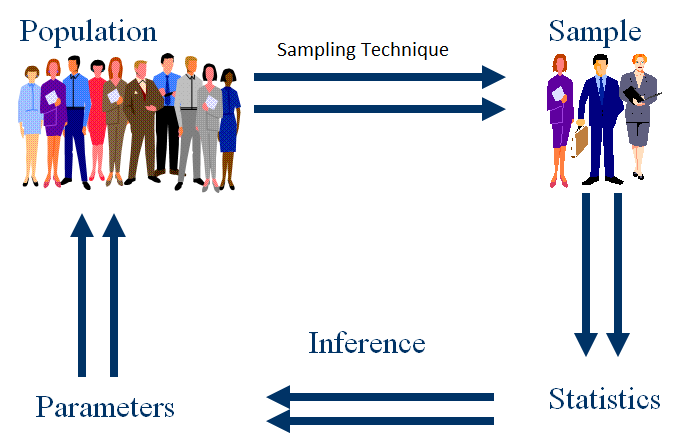
\includegraphics[scale=0.55]{paradigm}
\end{center}

\textsubscript{\textbackslash{}}\textbackslash{}\textsubscript{\textbackslash{}}\textbackslash{}
\textbf{Gas Example:}\textbackslash{} What is the population, sample,
parameter of interest, and statistic (most likely to be used)?

\newpage

Common Notation in statistics:

\begin{center}
\begin{tabular}{c|ccc}
Name & Parameter & Statistic & Quantity Measured\\
\hline
&&&\\
Mean & $\mu$ & $\bar{Y}$ or $\bar{y}$ or $\bar{X}$ or $\bar{x}$ & Center or Location\\
&&&\\
Proportion & $p$ or $\pi$ & $\hat{P}$ or $\hat{p}$ or $\hat{\pi}$ & Location or Frequency\\
&&&\\
Standard Deviation (SD) & $\sigma$ & $S$ or $s$ & Variability or spread\\
&&&\\
Variance (Var) & $\sigma^2$ & $S^2$ or $s^2$ & Variability or spread\\
\end{tabular}
\end{center}

\textasciitilde{}\textbackslash{} Note:
\(\bar{Y}=\frac{1}{n}\sum_{i=1}^{n}Y_i\) and
\(S^2=\frac{1}{n-1}\sum_{i=1}^{n}(Y_i-\bar{Y})^2\) where \(n\) is the
sample size (or number of observed values in the
sample).\textbackslash{}\textasciitilde{}\textbackslash{} Many, many,
many, more to come!
\textbackslash{}\textsubscript{\textbackslash{}}\textbackslash{}

Question of interest will lead you to which parameter you have interest
in. This will also most likely lead you to which type of data you will
collect.\textbackslash{}\textasciitilde{}\textbackslash{}

\textbf{Scales (Types) of Data:}\textbackslash{}

\begin{itemize}
\item \underbar{~~~~~~~~~~~~~~~~~~~~~~~~~~~~~~~~~~~~~~~~~~~~~~~~~} - A variable that is described by attributes or labels\\
\indent Subscales: \\
Nominal - categories have no ordering (Male, Female) (zip codes)\\
Ordinal - can order categories (Lickert scale data) (college football rankings)\\~\\
\item \underbar{~~~~~~~~~~~~~~~~~~~~~~~~~~~~~~~} - A variable that is described by numerical measurements where arithmetic can be performed\\
\indent Subscales: \\
Discrete - finite or countable finite number of values (\# of flowers on a plant, 0, 1, 2, ...)\\
Continuous - any value in an interval is possible (Temperature, $(-459.67\deg F, \infty)$\\
(Some lump these together and call them interval.)
\end{itemize}

\textasciitilde{}\textbackslash{} How we summarize and analyze the data
will depend on which type of data we have.

\newpage

\textbf{ex: SAT (get to know each other a little!)}\textbackslash{}

\begin{itemize}
\item 50 total students (16 males and 34 females) where matched on socio-economic background (all had similar income). 
\item A study was done to examine the effect of preparation atmosphere on SAT scores.  
\item Two types of atmospheres were investigated (strict vs easy going).
\item Students were divided into two groups of 25 (12 males and 13 females in strict class and 4 males 21 females in the easy going class).
\item After a 9 week tutoring session the SAT was taken (although 1 in the strict group did not take the exam and 5 in the easy going group did not take the exam).
\end{itemize}

With a partner or two (introduce yourselves):

\begin{enumerate}
\item Determine the research question.
\item Define the population and sample.
\item Define possible parameter(s) of interest.
\item Define possible statistics that might be calculated.
\item Why might the students have been matched on socio-economic background?
\item What issues might you see with the design of this study?
\item What other variables might you collect?
\end{enumerate}

\normalsize This class is about analyzing data. As scientists, most of
the time this data will come from a designed experiment, but the methods
used for analysis are also useful for observational studies. However,
the conclusions drawn will differ! Let`s define what me mean by
experimental and observational
study.\textbackslash{}\textasciitilde{}\textbackslash{}

\textcolor{red}{Observational Study}
\%\underbar{~~~~~~~~~~~~~~~~~~~~~~~~~~~~~~~~~~~~} researchers does not
interfere or intervene in the process of collecting data.

\begin{itemize}
\item Ex: measuring political beliefs in using a poll, measuring yield of a crop based on rainfall\\~\\~\\
\end{itemize}

\underbar{~~~~~~~~~~~~~~~~~~~~~~~~~~~~~~~~~~~~} researchers manipulate
the conditions in which the experiment is done.

\begin{itemize}
\item Ex: assigning different fertilizers and irrigation method and measuring crop yield, assigning temperatures of water to tanks containing a fish and observing weight gain
\end{itemize}

\textasciitilde{}\textbackslash{} Big difference in conclusions drawn!

\begin{itemize}
\item Cannot usually infer causation from observational experiments, but you can from a well-designed experiment.
\item Experiments are not always feasible or ethical.  i.e. cannot assign people to smoke a pack a day or have expectant mothers drink a certain amount of alcohol.
\end{itemize}

\textsubscript{\textbackslash{}}\textbackslash{} To describe the methods
for creating a well-designed experiment, we first need some definitions.

\begin{itemize}
\item \textbf{Response Variable} - Variable of interest that characterizes performance or behavior.
\item \textbf{Explanatory Variables} - Variables that determine the study conditions (can be quantitative or categorical).
\item \textbf{Factor} - Explanatory variable of interest.
\item \textbf{Level} -  The specified value of a factor (or explanatory variable).
\item \textbf{Confounding Variable} - Explanatory variable (not of interest) that may mask (or enhance) the effect of a factor.
\item \textbf{Covariate} - Quantitative confounding variable.
\item \textbf{Treatment} - A specific experimental condition, either the level of a factor (if only 1 factor) or the combinations of levels from a number of factors.
\item \textbf{Experimental units (EUs)} - Units on which the treatments are assigned.
\item \textbf{Measurement (Observational) units} - Units on which values are observed (often the same as EUs, but not always).
\item \textbf{Replicate} - Name given to EUs that receive the same treatment.
\item \textbf{Control Treatment} - Benchmark treatment sometimes necessary for comparison (to avoid the \textit{placebo effect}).
\item \textbf{Experimental Error} - Used to describe the variation in response among EUs that are assigned the same treatment.
\end{itemize}

\textbf{Example: } An experiment was run to determine the effects of
adding phosphorous (\(0, 147, 294, 441\) \(kg/m^2\)) and nitrogen
(\(0, 45, 90, 135\) \(kg/m^2\)) to the soil of a certain type of grass
(a Miscanthus species). The growth of the plant was of interest and at
the end of the growing period the plant was dried and the weight
recorded with the final measurement being recorded in megagram per
hectare (\(0.1\) \(kg/m^2\)). Four plots of grass were used in total.
Within each plot, each combination of phosphorous and nitrogen was
observed. The plots were arranged in a large field in a 4x1 rectangle
(north to south). There is a possibility of a water gradient as a stream
runs to the north of the field. A partial data table is given here:

\begin{center}
\begin{tabular}{c|c|c|c}
\hline
Plot    &P  &N& Dry yield\\
\hline
1&  0&  135&    1.95\\
1&  0&  45& 3.51\\
1&  0&  90& 2.87\\
1&  0&  0&  2.88\\
1&  294 &45&    2.37\\
1&  294 &0& 3.5\\
1&  294 &135&   3.55\\
1&  294&    90& 4.4\\
...&...&...&...\\
\end{tabular}
\end{center}

Let`s identify (if possible) the response, explanatory variable(s),
factor(s), level(s), confounding variable(s), treatment(s), number of
replicates, experimental units, and observational units.
\textbackslash{}\textsubscript{\textbackslash{}}\textbackslash{}\textsubscript{\textbackslash{}}\textbackslash{}\textsubscript{\textbackslash{}}\textbackslash{}\textsubscript{\textbackslash{}}\textbackslash{}\textsubscript{\textbackslash{}}\textbackslash{}\textsubscript{\textbackslash{}}\textbackslash{}\textasciitilde{}\textbackslash{}
(See example 2.4/2.7 and the resulting discussion for more practice)

\newpage

Notice that many of the response values are different. What is causing
them to be different?\textbackslash{}\textasciitilde{}\textbackslash{}
Sources of Variation in the responses of an experiment:

\begin{enumerate}
\item \textbf{Treatment effect} - we hope there is an effect due to the variables we are setting
\item \textbf{Identified confounding variables} - We record some variables that are not of interest, but we think may have an effect on the response.
\item \textbf{Unidentified sources (these make up the Experimental Error or error variation)} -
        \begin{enumerate}
            \item Inherent variability in experimental units - Experimental units are different! \\
        Ex: No two people, paper towels, concrete blocks, or even lab rats are exactly the same.\\
        Consequence: Experimental units respond differently to the same treatment
            \item Measurement error - Multiple measurements of a same experimental unit typically contain error.\\
            If the same experimental unit is measured more than once, will the value be the same?\\
            Ex: Blood Pressure, Break a water sample in two, measure each for bacteria
            \item Variations in applying/creating treatments\\
        The treatment is not clearly defined, leaving room for interpretation.  \\
            Ex:  Two researchers mix concrete, one stirs for 10 minutes and one for 20 minutes, will they come out exactly the same? Temperature is of interest but two ovens don`t heat exactly the same, etc.
            \item Effects from any other extraneous (or lurking) variables - Extraneous variables are those variables that are not part of the treatment, but may influence the response.\\
            Ex: For the oven example, the experiment is done over the course of several days.  There may be slight differences due to humidity changes.
        \end{enumerate}
\end{enumerate}

Let`s identify these in the grass growth example.
\textbackslash{}\textsubscript{\textbackslash{}}\textbackslash{}\textsubscript{\textbackslash{}}\textbackslash{}\textsubscript{\textbackslash{}}\textbackslash{}\textsubscript{\textbackslash{}}\textbackslash{}\textsubscript{\textbackslash{}}\textbackslash{}\textsubscript{\textbackslash{}}\textbackslash{}\textsubscript{\textbackslash{}}\textbackslash{}\textsubscript{\textbackslash{}}\textbackslash{}\textsubscript{\textbackslash{}}\textbackslash{}\textsubscript{\textbackslash{}}\textbackslash{}\textsubscript{\textbackslash{}}\textbackslash{}\textasciitilde{}\textbackslash{}
(See example 2.5/2.6 and the resulting discussion for more practice)

\newpage

No matter how hard we try, some experimental error will remain. What we
can do is use good experimental design techniques to ensure our study is
valid.\textbackslash{}\textasciitilde{}\textbackslash{} DOE is about
creating the optimal experiment to determine the effects of different
treatments. Different types of experimental designs are then analyzed
differently.\textbackslash{}\textasciitilde{}\textbackslash{}
\textbf{Pillars of Experimental Design}\textbackslash{}

\begin{enumerate}
        \item \underbar{~~~~~~~~~~~~~~~~~~~~~~~~~~~~~} - means that the treatments are randomly allocated to the EUs.
            \begin{enumerate}
                \item Every EU has a chance to get a different treatment, so helps protect the results of the analysis against a systematic influence of lurking variables.  
                \item Allows the observed responses to be regarded as a random sample.
            \end{enumerate}
        Note: Different randomization schemes lead to different statistical analyses.\\~\\
        \underbar{~~~~~~~~~~~~~~~~~~~~~~~~~~~~~~~~~~~~~~~~~~~~~~~~} - for t treatments, replicated $n_t$ times each, use a random number generator to assign the treatments to the EUs.\\~\\
        Most basic randomization design - assumes all EUs are exchangeable.\\~\\~\\~\\~\\~\\~\\~\\~\\
        \item \underbar{~~~~~~~~~~~~~~~~~~~~~~~~~~~~~} - Repetition of an experiment using a large group of subjects to reduce chance variation in the results
\begin{enumerate}
                \item Allows us to generalize the results to the population and increases reliability of conclusions. 
                \item Allows an estimate of variability (an estimate of experimental error) not due to the treatment effect.
            \end{enumerate}
Note: Replication does not mean that we measure the same EUs multiple times, this is called repeated measures.  Observations from repeated measures experiments cannot  usually be considered independent.
%\noindent\textit{Ideally as many EUs as we can afford.  Think if we had 3 diets and 3 EUs.  Diet 1 was better than diet 2 and diet 3, not a very reliable conclusion, perhaps person 1 just loses weight more easily.  Now if 100 people at each diet and on average diet 1 was much better, more reliable conclusion.}\\~\\
%\noindent\textit{By averaging over the many observations we can reduce the effects of measurement error and error in applying/creating the treatments.}\\~\\
\newpage
        \item \textbf{Methods for accounting for/reducing experimental error}
        \begin{enumerate}
            \item Controlling Variables - holding certain variables constant across the EUs\\
            Decreases generalizability, but reduces experimental error.\\~\\
\noindent\textit{We`re not interested in the effects of these variables on the response.  These variables affect the response in exactly the same manner, so that we    don`t see the effects on the conclusions. We don`t get information on what happens at levels other than the fixed one.}
        \item Blocking - Divide subjects with similar characteristics into `blocks', and then within each block, randomly assign subjects to treatment groups.\\~\\
            Blocks - Groups of EUs sharing a common level of a confounding variable.\\
\begin{center}
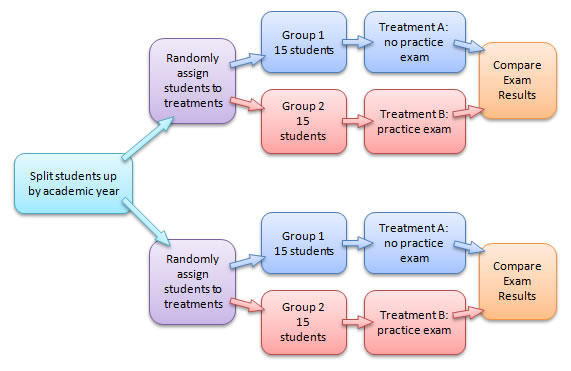
\includegraphics[scale=0.5]{block.jpg}
\end{center}
            Similar to controlling, but allows for increased generalizability.  EUs within a block are very similar (decreases experimental error there as all the EUs in a block are affected similarly by the confounding variable).  By having enough blocks to cover the range of the population you can still generalize.)
        \end{enumerate}
    \end{enumerate}

\noindent\textit{There are also methods for dealing with some explained experimental error during the analysis stage - Namely ANCOVA.\\~\\
        These ideas are very important.  Unless you are well versed in statistical methods and ideas you should consult a statistician before investing time and money in an experiment.\\
`A poorly designed study can never be saved, but a poorly analyzed one has the possibility of being reanalyzed.'}

\normalsize \textbackslash{}\textasciitilde{}\textbackslash{} Recall:
Process of a study involves

\begin{enumerate}
\item Identify the research objective
\item Collect the information needed to answer the questions
\item Organize and summarize the information.
\item Draw conclusions from the information.
\end{enumerate}

We will now talk about step
3!\textbackslash{}\textasciitilde{}\textbackslash{} So you have
data\ldots{} now what??\textbackslash{}

\begin{center}
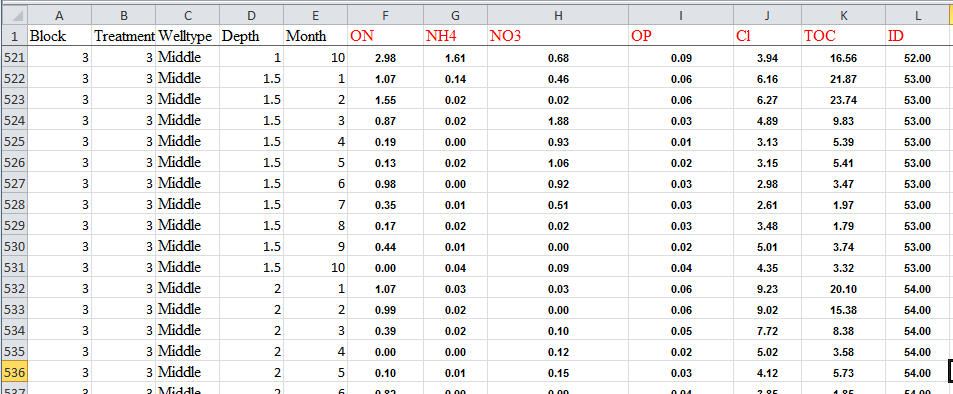
\includegraphics[scale=0.7]{spreadsheet}
\end{center}

Whether we are describing an observed population or using sampled data
to draw an inference from the sample to the population, an insightful
description of the data is an important step in drawing conclusions from
it. \textbackslash{}\textasciitilde{}\textbackslash{}

Good descriptive statistics enable us to make sense of the data by
reducing a large set of measurements to a few summary measures that
provide a good, rough picture of the original
measurements.\textbackslash{}\textasciitilde{}\textbackslash{}

Summary measure used for a variable depends on its
\underbar{~~~~~~~~~~~~~~~~~~~~~~~~~~~~~~~~~~~~}.\textbackslash{}\textasciitilde{}\textbackslash{}

Our goal will be to describe the variable's
\underbar{~~~~~~~~~~~~~~~~~~~~~~~~~~~~~~~~~~~~}\textbackslash{}\textasciitilde{}\textbackslash{}
i.e.~the \textbackslash{}\textasciitilde{}\textbackslash{}

Two major characteristics of the variable's distribution that we often
describe are
\underbar{~~~~~~~~~~~~~~~~~~~~~~~~~~~~~~~~~~~~}\textbackslash{}\textasciitilde{}\textbackslash{}
and
\underbar{~~~~~~~~~~~~~~~~~~~~~~~~~~~~~~~~~~~~}\textbackslash{}\textasciitilde{}\textbackslash{}

We will mostly deal with quantitative variables and our focus will be on
their summary measures. However, we will briefly talk about graphs and
statistics for categorical
variables.\textbackslash{}\textasciitilde{}\textbackslash{}

\huge Categorical Variables \normalsize\textbackslash{} Numerical
measure used for categorical
variable:\textbackslash{}\textsubscript{\textbackslash{}}\textbackslash{}\textsubscript{\textbackslash{}}\textbackslash{}
For this simple study, we can find the sample proportion for each
categorical variable:\textbackslash{}
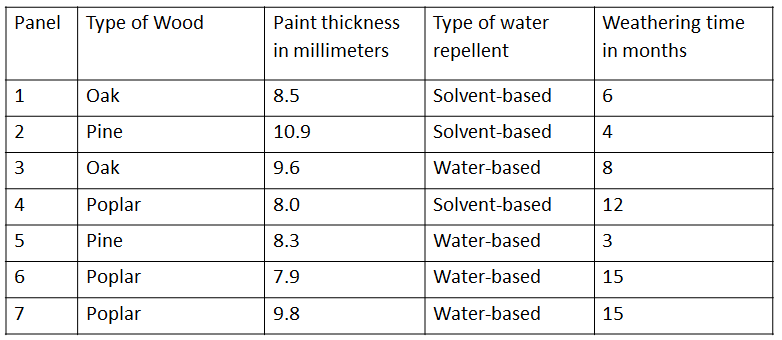
\includegraphics[scale=0.5]{paintexample}

\newpage

The main plots used are \underbar{~~~~~~~~~~~~~~~~~~~~~~~~~~~~~~~~~~~~}
and
\underbar{~~~~~~~~~~~~~~~~~~~~~~~~~~~~~~~~~~~~}.\textbackslash{}\textasciitilde{}\textbackslash{}

\underbar{~~~~~~~~~~~~~~~~~~~~~~~~~~~~~~~~~~~~} - use percents to
display data.

\begin{itemize}
\item Order does not matter (although should order from highest percentage to lowest)
\end{itemize}

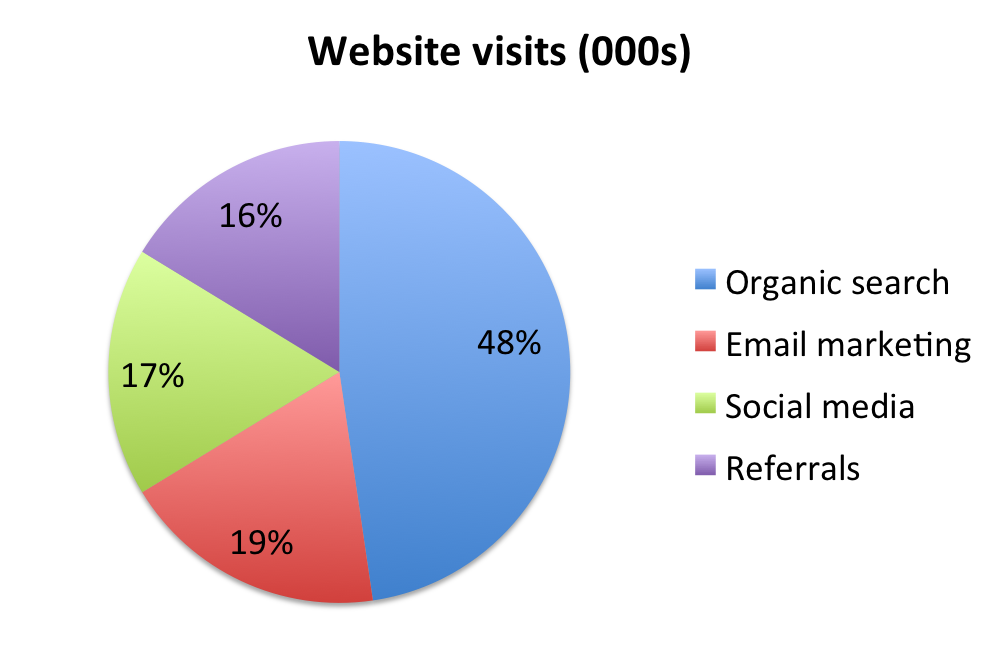
\includegraphics[scale=0.5]{piechart}\textbackslash{}
\underbar{~~~~~~~~~~~~~~~~~~~~~~~~~~~~~~~~~~~~} - Categories along the
x-axis. Count, percent, or relative frequency (sample proportion) along
the y-axis.\\

\begin{itemize}
\item Order does not matter (although should order from highest percentage to lowest).  
\item A gap should exist between the bars.
\end{itemize}

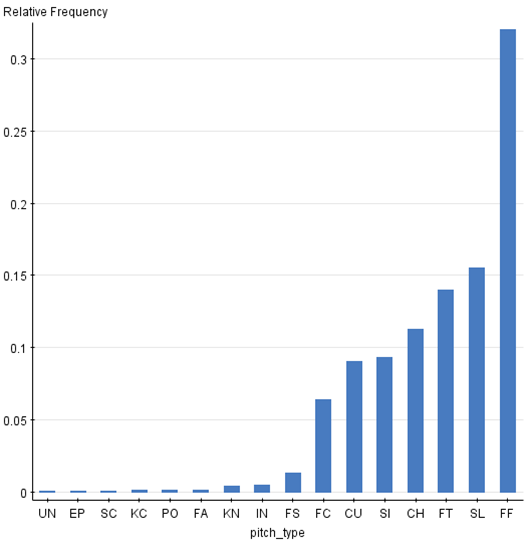
\includegraphics[scale=0.5]{bargraph}

\newpage

We might also have multiple categorical variables of interest. In which
case, a good display of the data
is\textbackslash{}\textasciitilde{}\textbackslash{} a
\underbar{~~~~~~~~~~~~~~~~~~~~~~~~~~~~~~~~~~~~~~~~~~~~~~~~~~~~~}.\textbackslash{}\textasciitilde{}\textbackslash{}
Let's create one for the paint example from
earlier.\textbackslash{}\textsubscript{\textbackslash{}}\textbackslash{}\textsubscript{\textbackslash{}}\textbackslash{}\textsubscript{\textbackslash{}}\textbackslash{}\textsubscript{\textbackslash{}}\textbackslash{}\textsubscript{\textbackslash{}}\textbackslash{}\textasciitilde{}\textbackslash{}

Book example on page 103 is nice.
\textbackslash{}\textasciitilde{}\textbackslash{}

Many other methods exist such as comparative bar
charts:\textbackslash{}\textsubscript{\textbackslash{}
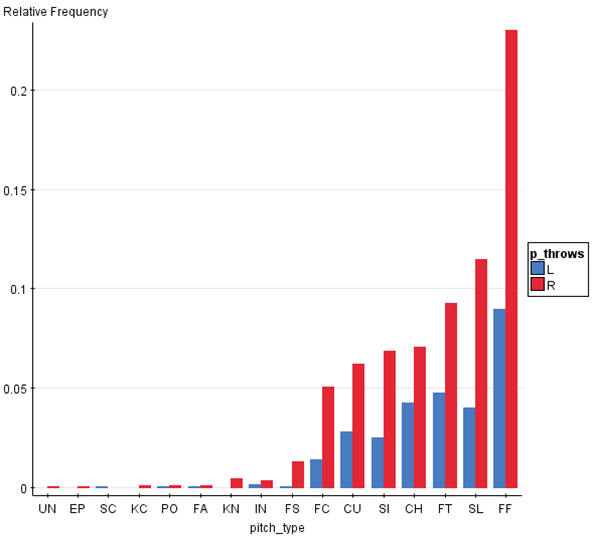
\includegraphics[scale=0.5]{bargraph2}\textbackslash{}}\textbackslash{}

\newpage

\huge Quantitative Variables \normalsize\textbackslash{} We will again
consider the paint example:\textbackslash{}
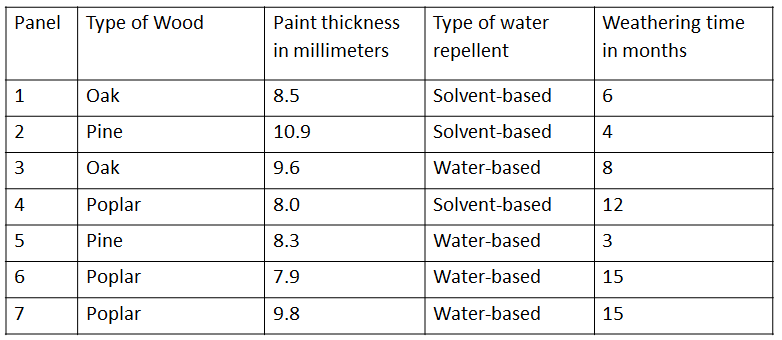
\includegraphics[scale=0.5]{paintexample}\textbackslash{} Numerical
measures of
location:\textbackslash{}\textsubscript{\textbackslash{}}\textbackslash{}\textsubscript{\textbackslash{}}\textbackslash{}\textsubscript{\textbackslash{}}\textbackslash{}\textsubscript{\textbackslash{}}\textbackslash{}\textsubscript{\textbackslash{}}\textbackslash{}\textsubscript{\textbackslash{}}\textbackslash{}\textsubscript{\textbackslash{}}\textbackslash{}\textsubscript{\textbackslash{}}\textbackslash{}\textsubscript{\textbackslash{}}\textbackslash{}\textasciitilde{}\textbackslash{}
\newpage
Numerical Measures of Spread \newpage
The main plots used are \underbar{~~~~~~~~~~~~~~~~~~~~~~~~~~~~~~~~~~~~}
and
\underbar{~~~~~~~~~~~~~~~~~~~~~~~~~~~~~~~~~~~~}.\textbackslash{}\textasciitilde{}\textbackslash{}

A \underbar{~~~~~~~~~~~~~~~~~~~~~~~~~~~~~~~~~~~~} is obtained by
splitting the range of the data into equal-sized bins. Then for each
bin, we count the number of points that fall into each bin and that is
the height of our bar (or use relative frequency - i.e.~proportion in
category).\\

\begin{itemize}
\item Typically, an observation equal to a boundary value is put in the higher interval.
\item Bars should touch!
\item Too many classes will spread the data out, thereby not revealing the pattern.  Too few classes will lump the data.  
\item **** This is the most important graphical technique for displaying the distribution of a quantitative variable!
\end{itemize}

Ex. Ages of the winners of the best actress Academy Award in the recent
20 years (1994-2013) are: 36, 45, 49, 39, 34, 26, 25, 33, 35, 35, 28,
30, 29, 61, 32, 33, 45,29, 62 and 22\textbackslash{}
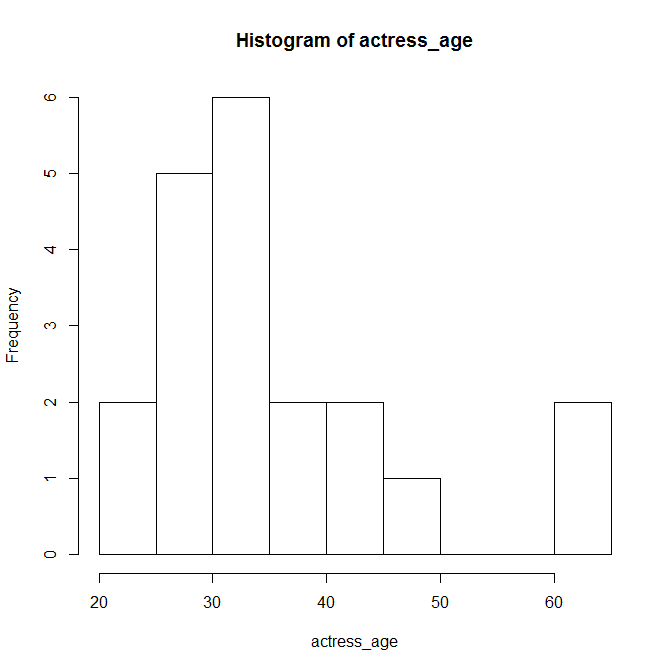
\includegraphics[scale=0.3]{oscarhist}\textbackslash{}

What are we looking for in a histogram?\textbackslash{}

\begin{itemize}
\item ~\\
\item ~\\
\item ~
\end{itemize}\newpage

Relationship between mean and median for a histogram (note pictures use
smooth curves, but same ideas hold):\textbackslash{}
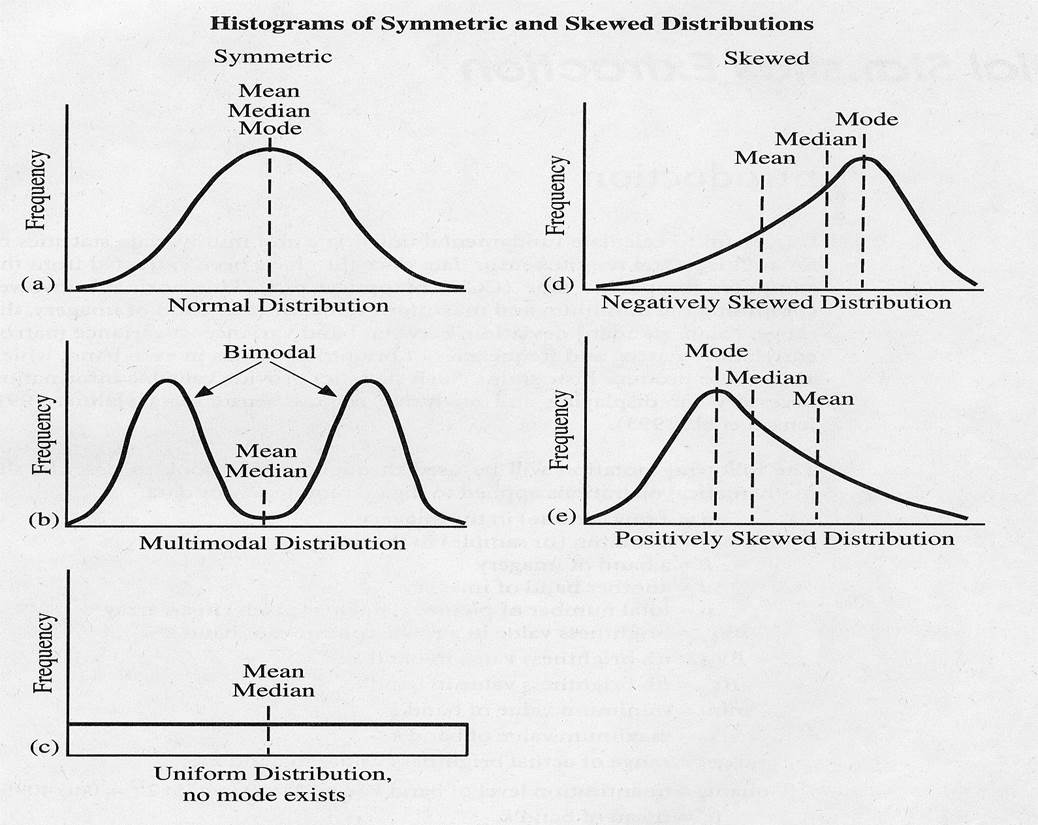
\includegraphics[scale=0.6]{meanmedianrelationship}\textbackslash{}

A \underbar{~~~~~~~~~~~~~~~~~~~~~~~~~~~~~~~~~~~~} displays the five
number summary of the
data.\textbackslash{}\textasciitilde{}\textbackslash{} Five number
summary
includes:\textbackslash{}\textsubscript{\textbackslash{}}\textbackslash{}\textasciitilde{}\textbackslash{}

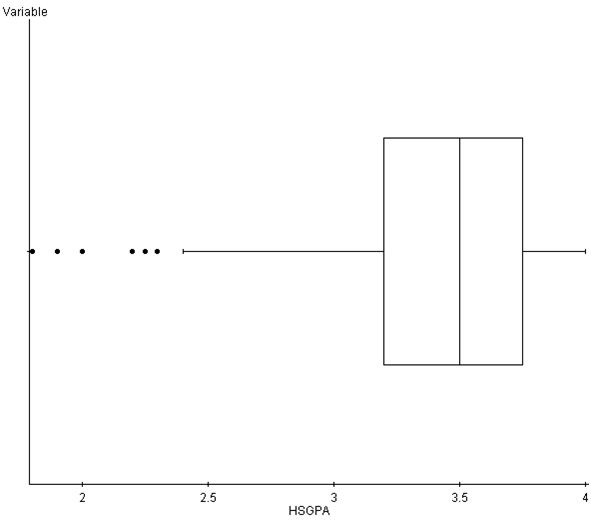
\includegraphics[scale=0.5]{boxplot2}\textbackslash{}

\begin{itemize}
\item Measure of center from a boxplot - \\
\item Measures of spread from a boxplot - \\~\\
\item Can tell skewness but not modality!
\end{itemize}

If we have two quantitative variables of interest, we often look at
\underbar{~~~~~~~~~~~~~~~~~~~~~~~~~~~~~~~~~~~~~~~~~~~~~~~~~~~~~}
\textbackslash{}\textasciitilde{}\textbackslash{} and
\underbar{~~~~~~~~~~~~~~~~~~~~~~~~~~~~~~~~~~~~~~~~~~~~~~~~~~~~~} to
inspect the `linear association' between the variables (call them x and
y).\textbackslash{}
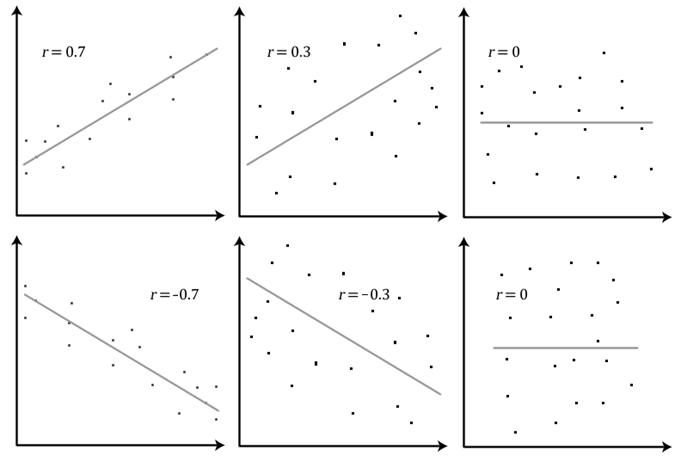
\includegraphics[scale=0.6]{scatterplots}\textbackslash{} We will look
at these more later in the
course.\textbackslash{}\textsubscript{\textbackslash{}}\textbackslash{}
If we have a quantitative and a categorical variable, we often look at
\underbar{~~~~~~~~~~~~~~~~~~~~~~~~~~~~~~~~~~~~~~~~~~~~~~~~~~~~~}.\textbackslash{}
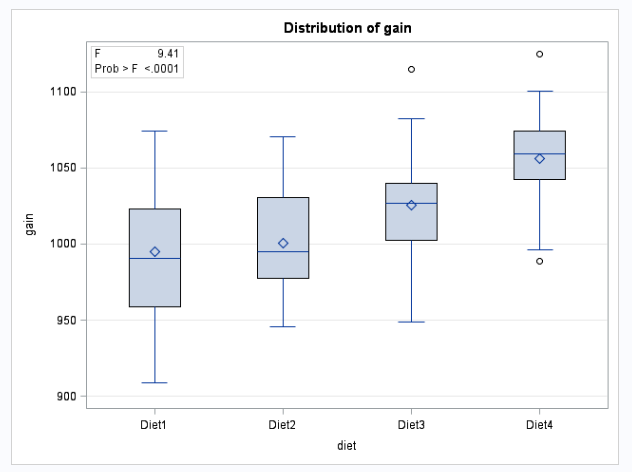
\includegraphics[scale=0.6]{ChickensBoxPlot}\textbackslash{}\textasciitilde{}\textbackslash{}
Review - \textbackslash{} Numeric Summaries of Location:
Mean/median/trimmed mean (quantitative), proportion
(qualitative)\textbackslash{} Numeric Summaries of Spread: Variance, SD,
IQR, CV, Quartiles (quantitative)\textbackslash{} Graphical Summaries
for categorical: Bar Chart, Pie Graph\textbackslash{} Graphical
Summaries for quantitative: Histogram, Boxplot

\chapter{Point Estimates}\label{point-estimates}

Learning objectives for this lesson: - How to estimate a mean -
Definition of ``convenience sample'' - Definition of ``systematic
sample'' - Benefits/drawbacks to both approaches - Understand how to
estimate a mean - Understand how to estimate a quantile - Understand
implicit assumptions for these approaches

\section{Estiamte with means}\label{estiamte-with-means}

\subsection{Experiment background}\label{experiment-background-2}

Someone wants to know how much of something they need to satisfy some
population To get a good estimate of this, we can use the average amount
for each one and then multiply by the whole population

\section{Estimate with quantiles}\label{estimate-with-quantiles}

\subsection{Experiment background}\label{experiment-background-3}

Big Deborah's is making new packaging for their cookies. The engineer
responsible for the new desing needs to make sure that the packaging
fits the new cookies. While the cookie manufacturing process is
standardized, there's inevitably some degree of variation in cookie
size. After discussing the issue with corporate, the engineer decides
that a the new cookie sleeves should be large enough to fit 95\% of
cookies that are baked. (The largest five percent will be marketed
separately as ``JUMBO'' cookies.)

\subsection{Define the object of the
experiment}\label{define-the-object-of-the-experiment}

The Engineer is tasked with determining how large the cooke sleeve needs
to be. There's no way for her to know the size of every cookie that Big
Deborah's has made (or will make going forward!), so she'll need to
collect data on existing cookies to inform her cookie sleeve size
determination.

\subsection{Select appropriate response
variables}\label{select-appropriate-response-variables}

If the maximum distance from any one point on the (round) cookie's
perimeter to any other point is smaller than the diameter of the cookie
sleeve, then the cookie will fit. This makes ``cookie diameter'' a good
measure for this test. It is easy to measure for each cookie and is
directly relevant to the experiment's objective.

{[}probably have something in here about {]}

\subsection{IDentify sources of
variation}\label{identify-sources-of-variation}

While the manufacturing process is standardized, there is variation in
size from one cookie to the next. This is one source of variation. The
engineer isn't sure of any others. However, she knows that cookies are
made in multiple factories, and that each factory has multiple ovens.
Ovens and factories could also be sources of variation.

\subsection{Choose an experimental
design}\label{choose-an-experimental-design-2}

The Engineer knows that she needs to look at multiple cookies, since she
knows that there is variation in diameter from one cookie to the next.
One option would be to just use the remaining cookies in the box she has
in her office (22 of the 25-count box remain). {[}something about
convenience sample{]} However, she knows that cookies from the same oven
are typically packaged together. If there is variation from one oven to
the next, looking at the cookies she has in her office may not tell the
whole story.

Instead, she chooses to take every 20th cookie manufactured off the
assembly line until she gets 500 cookies. {[}something about systematic
sample{]}

\subsection{Perform the test}\label{perform-the-test}

The day of the test comes, and the Engineer starts collecting cookies.
However, problems arise! The plan has to shut down half-way through, so
she only gets 431 cookies instead of the 500 she thought she would.
However, she measures the diameters of each cookie and records the data
in a spreadsheet.

\subsection{Statistically analyze the
data}\label{statistically-analyze-the-data-2}

The initial plan had been to rank-order the 500 cookies and estimate the
95th percentile using the diamter of the 475th largets cookie. Since we
didn't get all of our data, we have to improvise. 431 doesn't neatly
yield a value such that exactly 95\% are less than or equal and 5\% are
greater than or equal. One option is to choose the 410th largest cookie
to estimate our percentile. Slightly more than 95\% of cookies will have
smaller diameters than this. Alternatively, we could interpolate between
the 409th and 410th cookies. {[}reasons and logic and math for each of
these{]}

\subsection{Draw conclusions}\label{draw-conclusions-2}

Based on this study, the Engineer concludes that a cookie sleeve large
enough for a cookie of diameter XX will be big enough to contain 95\% of
Big Deborah cookies.

\subsection{Discussion}\label{discussion}

\begin{itemize}
\tightlist
\item
  pros and cons to the approach chosen
\item
  generalizing to other types of point estimates
\end{itemize}

\chapter{Accounting for Uncertainty}\label{accounting-for-uncertainty}

Some \emph{significant} applications are demonstrated in this chapter.

\section{Example one}\label{example-one}

\section{Example two}\label{example-two}

\chapter{Inference via Hypothesis Tests for One Sample}\label{HT}

We have finished a nice book.

\chapter{Inference via Confidence Intervals for One Sample}\label{CI}

We have finished a nice book.

\chapter{Inference for Two Categorical Variables}\label{twocategorical}

We have finished a nice book.

\chapter{One-Way ANOVA}\label{anova}

Learning objectives for this lesson: - Write one-way ANOVA model -
Define terms - state assumptions - interpret results - Interpret ANOVA
table - Describe SSE, SST, MSE - F-statistic - degrees of freedom -
understand how all of these interrelate - Understand how to compare
mulitple group means how ANOVA is similar/different to t-tests -
Understand partitioning of variation and coefficient of determination

\chapter{Motivating example}\label{motivating-example}

The United States Air Force Academy has 24 sections of Calculus I,
taught by three different types of instructors: In-uniform instructors,
full-time civilian instructors, and visiting faculty. The Dean of
Students wants to give students the best experience possible and make
sure that all three types of instructors are doing a good job. There are
plausible reasons why any one of the three could be doing well:
In-uniform instructors are all members of the Air Force, and students
may be extra attention in these classes because they know that these
instructors rank above them in their chain of command. On the other
hand, full-time instructors have been aroudn the Academy for many years
and understand the Cadets and their workloads. Alternatively, visiting
facutly tend to come from prestigeous institutions and may be familiar
with more recently-developed pedagogical techniques. Regardless, the
Dean wants to understand if there is any variation in end-of-semester
grades of classes taught by these three types of instructors. At the end
of the semester, she collects the average grades from each of the 24
sections. How can she go about investigating this question?

Recall from Chapter 6 that we can use t-tests to compare two group
means. In this case, we'd like to do a comparison across three groups,
and instead of looking at a direct comparison of one group to another,
what the Dean is interested in is whether there's an \emph{overall}
difference across the three groups.

One option might be to just do a bunch of different t-tests. We could
first compare classes taught by in-uniform instructors to classes taught
by full-time civilians, then compare the classes taught by the
in-uniform instructors to the classes taugth by the visiting
instructors, and then finally compare the classes taugth by the
full-time civilains with the classes taught by the visiting facutly.
We'd end up with three p-values, each addressing different questions
than the one we initially set out to answer.

We could do the same thing, except comparing courses taught by one type
of instructor to the combined group of courses taught by the other two,
and this gets a bit closer to the mark. But we're still doing three
tests that individually fail to answer the Dean's question.

What we'd like instead is a single hypothesis that we could test that
direclty gets at the Dean's concern about whether the three types of
instructors were producing end-of-semester grades that were, on average,
the same. {[}Need to make that motivation clearer above.{]}

\chapter{Simple model for the data}\label{simple-model-for-the-data}

Narrative explanation that instructor type might matter, there shold be
some variation from class to class. - write some things in greek,
including model without any difference by instructor type - wirte model
with differences by instructor type - note that we can use Gaussian
errors b/c Academy grades do actually tend to be centered around a C,
particularly for classes like Calc - discuss model assumptions in
general sense

\chapter{exploratory analysis}\label{exploratory-analysis}

\begin{itemize}
\tightlist
\item
  course-to-course variability is expected
\item
  maybe show a plot of it or something
\item
  visualize groups using box-and-whisker plots
\end{itemize}

\chapter{sources of variation}\label{sources-of-variation}

Things like student population, time of day, etc. But we'll throw this
all into an error term and focus on the main one, instructor type

\chapter{statistical model and
analysis}\label{statistical-model-and-analysis}

\begin{itemize}
\tightlist
\item
  ANVOA model explicit w/ assumptions
\item
  variation around overall mean w/ no groups
\item
  variation around group means
\item
  introduce idea of reference level
\end{itemize}

\chapter{compare analyses}\label{compare-analyses}

\begin{itemize}
\tightlist
\item
  t-test methods from above
\item
  ANOVA method
\item
  compare and contrast results, interpretations, etc.
\end{itemize}

\chapter{Multi-way ANOVA}\label{multiway}

We have finished a nice book.

\chapter{Block Designs}\label{block}

We have finished a nice book.

\chapter{Regression Models}\label{regression}

We have finished a nice book.

\chapter{The General Linear Model}\label{glm}

We have finished a nice book.

\chapter{Mixed Models}\label{mixedmodels}

We have finished a nice book.

\chapter{Split Plot and Repeated Measures
Designs}\label{repeatedmeasures}

We have finished a nice book.

\chapter{Logistic Regression and Generalized Linear
Models}\label{logistic}

\section{Stuff here}\label{stuff-here}

We have finished a nice book.

\chapter{Generalized Linear Mixed Models}\label{glmm}

We have finished a nice book.

\chapter{Appendix - Learning Objectives}\label{learningobj}

\section{Book-level}\label{book-level}

After reading this book you will be able to:

\begin{itemize}
\item
  identify relevent sources of variability for a potential study and, if
  applicable, utilize principles of design to plan a reasonable
  experiment to help answer questions of interest

  \begin{itemize}
  \tightlist
  \item
    covariates
  \item
    noise variables
  \item
    random effects
  \item
    variance of indidvidual observations vice variance of summary
    statistics
  \item
    randomization
  \item
    systematic variation of factors/covariates
  \item
    factor identifiability
  \item
    understand issues surrounding multiple comparisons

    \begin{itemize}
    \tightlist
    \item
      Bonferroni correction
    \item
      at least one other method (Tukey?)
    \end{itemize}
  \item
    tradeoffs from replication within groups vice getting more groups
  \item
    compare and contrast methods for designing an experiment when the
    goal of a study is prediction versus when the goal is statistical
    inference
  \end{itemize}
\item
  explain the general concept of point estimation and how to account for
  sampling variability

  \begin{itemize}
  \tightlist
  \item
    definition
  \item
    identify the right point estimate for your response variable of
    interest
  \item
    estimating uncertainty for point estimates

    \begin{itemize}
    \tightlist
    \item
      normal approximation
    \item
      bootstrap CI
    \item
      others?
    \end{itemize}
  \item
    Types of point estimates:

    \begin{itemize}
    \tightlist
    \item
      means

      \begin{itemize}
      \tightlist
      \item
        Simple effects
      \item
        interaction effects
      \item
        main effects
      \end{itemize}
    \item
      standard deviations/variance components
    \item
      correlation coefficients
    \item
      quantiles/percentiles from distributions
    \item
      probabilities
    \item
      parameters of a distribution
    \item
      model parameters
    \end{itemize}
  \end{itemize}
\item
  describe relevant properties of random variables and probabilities

  \begin{itemize}
  \tightlist
  \item
    Distinguish between mutually exclusive and independent events.
  \item
    Calculate probability for a given scenario, either numerically or
    using a Venn diagram.
  \item
    Apply the General Addition Rule to solve probability problems.
  \item
    Apply the Rules for Probability Distributions to create a
    probability distribution for a given scenario.
  \item
    Use the complement of an event to solve probability problems.
  \item
    Apply the Multiplication Rule for Independent Processes to solve
    probability problems.
  \item
    random variables

    \begin{itemize}
    \tightlist
    \item
      have a defined set of possible outcomes (``sample space'')
    \item
      Discrete vs.~continuous RVs
    \item
      others???
    \end{itemize}
  \item
    probabilities/PDFs

    \begin{itemize}
    \tightlist
    \item
      between 0 and 1 inclusive
    \item
      sum of probability of all possible events is 1
    \item
      \(P(A) + P(A^c) = 1\), where \(A\) is an event and \(A^c\) is the
      complement of A
    \end{itemize}
  \end{itemize}
\item
  explain the importance of statistical distributions when conducting
  statistical inference

  \begin{itemize}
  \tightlist
  \item
    normal distribution and approximations plus properties

    \begin{itemize}
    \tightlist
    \item
      robustness
    \item
      generality
    \item
      CLT
    \end{itemize}
  \item
    costs and benefits of using nonparametric approaches
  \end{itemize}
\item
  describe the fundamental inferential techniques of hypothesis testing
  and confidence intervals as well as compare and contrast their uses
  and interpretations
\item
  identify a null and alternative for a given problem

  \begin{itemize}
  \tightlist
  \item
    interpret hypotheses
  \item
    characterize the test statistic under the null
  \item
    explain what a rejection region and be able to identify one
  \item
    define statistical power
  \item
    calculate statistical power for one- and two-sample tests of
    continuous and binary random variables
  \item
    define statistical confidence\\
  \item
    identify when using a CI and NSHT will result in the same conclusion
  \item
    explain when you can use a confidence interval to test for
    differences (e.g., comparing a single point estimate to a threshold)
    and when you can't (e.g., when you have CIs for two different means)
  \end{itemize}
\item
  choose appropriate numerical summaries and graphical displays for a
  set of data and create these using software

  \begin{itemize}
  \tightlist
  \item
    when to use tables vs.~a picture
  \item
    types of graphical displays

    \begin{itemize}
    \tightlist
    \item
      bar charts
    \item
      pie charts
    \item
      plotting data vice just predictions/conclusions
    \item
      when to include uncertainty bounds
    \item
      five-number summaries
    \item
      means vs.~medians
    \item
      general plotting recommendations
    \item
      use of colors in you plots (discrete vs.~divergent vs.~continuous
      color scales, gray-scale, color-blind-friendly scales)
    \end{itemize}
  \item
    use of annotations
  \item
    general graphical design philosophy (building a chart to illustrate
    a conclusion)
  \item
    trade-offs between detail and interpretability
  \item
    not screwing up your axes
  \end{itemize}
\item
  fit statistical models in software and interpret their output

  \begin{itemize}
  \tightlist
  \item
    Which PROCs from SAS? REG, GLM, MIXED, GLIMMIX, others??
  \item
    \texttt{lm()}, \texttt{glm()}, \texttt{anova()} \ldots{}.
    \texttt{broom}? \texttt{modelr}? \texttt{ciTools}?
  \item
    p-values, point estimates, standard errors, f-statistics,
    chi-square-statistics, degrees of freedom, SS/MS, residual plots
  \end{itemize}
\item
  connect common statistical methods under the linear model framework

  \begin{itemize}
  \tightlist
  \item
    Write statistical models using matrix representaiton
  \item
    identify models written in matrix representation with their
    representation in software
  \item
    identify when models written in different notation are the same or
    different
  \item
    describe when specific models will give you the same results

    \begin{itemize}
    \tightlist
    \item
      ANOVA w/ 2 factors and a t-test or a SLR
    \item
      ANCOVA and MLR
    \item
      random effects vs.~fixed effects
    \item
      split plots vs.~more general mixed models
    \item
      logistic regression w/ categorical factors vice contingency table
      analysis
    \end{itemize}
  \item
    discuss differences in assumptions associated with ANOVA vice
    SLR/MLR
  \end{itemize}
\item
  articulate the scope of inferential conclusions in light of the method
  of data collection, the experimental design used, the assumptions
  made, and the statistical analysis applied

  \begin{itemize}
  \tightlist
  \item
    limitations due to sampling/sample frame
  \item
    missing data
  \item
    modeling assumptions
  \item
    sampling assumptions
  \item
    requirements for causal inference
  \end{itemize}
\end{itemize}

\section{Topic-level}\label{topic-level}

\subsection{Chapter 2 - Sampling, Design, and Exploratory Data
Analysis}\label{chapter-2---sampling-design-and-exploratory-data-analysis}

\subsection{Chapter 3 - Point
Estimation}\label{chapter-3---point-estimation}

\subsection{Chapter 4 - Accounting for Uncertainty in
Estimation}\label{chapter-4---accounting-for-uncertainty-in-estimation}

\subsection{Chapter 5 - Inference via Hypothesis Testing for a
Proportion or
Mean}\label{chapter-5---inference-via-hypothesis-testing-for-a-proportion-or-mean}

\subsection{Chapter 6 - Inference via Confidence Intervals for a
Proportion or
Mean}\label{chapter-6---inference-via-confidence-intervals-for-a-proportion-or-mean}

\subsection{Chapter 7 - Inference on Two Categorical
Variables}\label{chapter-7---inference-on-two-categorical-variables}

\subsection{Chapter 8 - Inference for Multiple
Means}\label{chapter-8---inference-for-multiple-means}

\subsection{Chapter 9 - Multiway
ANOVA}\label{chapter-9---multiway-anova}

\subsection{Chapter 10 - Block
Designs}\label{chapter-10---block-designs}

\subsection{Chapter 11 - Regression}\label{chapter-11---regression}

\subsection{Chapter 12 - The General Linear
Model}\label{chapter-12---the-general-linear-model}

\subsection{Chapter 13 - Mixed Models}\label{chapter-13---mixed-models}

\subsection{Chapter 14 - Repeated Measures and Split Plot
Designs}\label{chapter-14---repeated-measures-and-split-plot-designs}

\subsection{Chapter 15 - Logistic Regression and Generalized Linear
Models}\label{chapter-15---logistic-regression-and-generalized-linear-models}

\subsection{Chapter 16 - Generalized Linear Mixed
Models}\label{chapter-16---generalized-linear-mixed-models}

\section{From ST512}\label{from-st512}

WE NEED TO ORGANIZE THESE UNDER DIFFERENT CHAPTERS AT SOME POINT
Learning Objectives

\begin{enumerate}
\def\labelenumi{\arabic{enumi}.}
\item
  Recognize a completely randomized design with one treatment factor and
  write the corresponding one-way analysis of variance model, with
  assumptions
\item
  Estimate treatment means
\item
  Estimate the variance among replicates within a treatment
\item
  Construct the analysis of variance table for a one factor analysis of
  variance, including computing degrees of freedom, sums of squares,
  mean squares, and F-ratios
\item
  Interpret results and draw conclusions from a one-factor analysis of
  variance
\item
  Estimate differences between two treatment means in a one factor
  analysis of variance
\item
  Test differences between two treatment means in a one factor analysis
  of variance
\item
  Construct a contrast to estimate or test a linear combination of
  treatment means
\item
  Estimate the standard error of a linear combination of treatment means
\item
  Make inferences about linear combinations of treatment means,
  including contrasts.
\item
  Obtain and understand SAS output for linear combinations of treatment
  means, including contrasts.
\item
  Explain when and why corrections for multiple comparisons are needed
\item
  Know when and how to use Tukey's correction for all pairwise
  comparisons
\item
  Compute Bonferroni confidence intervals
\item
  Create and interpret orthogonal contrasts.
\item
  Define main effects and interactions
\item
  Write contrasts to estimate main effects and interactions
\item
  Estimate these contrasts and their standard errors
\item
  Compute sums of squares associated with these contrasts
\item
  Test hypotheses about the main effects and interactions.
\item
  Identify and define simple effects.
\item
  Identify and define interaction effects.
\item
  Identify and define main effects.
\item
  Understand when to use simple, interaction, and main effects when
  drawing inferences in a two-way ANOVA.
\item
  Write the analysis of variance model and SAS code for a completely
  randomized design with two factors
\item
  Test hypotheses and interpret the analysis of variance for a factorial
  experiment.
\item
  Explain the appropriate use of correlations and compute the
  correlation coefficient
\item
  Read and interpret a scatterplot and guess the correlation coefficient
  by examination of a scatter plot
\item
  Interpret the strength and direction of association indicated by the
  correlation coefficient and judge when a correlation coefficient
  provides an appropriate summary of a bivariate relationship
\item
  Test the hypothesis that the correlation coefficient is zero using
  either a t-test or the Fisher z transformation, Compute confidence
  intervals using Fisher's z transformation
\item
  Write a statistical model for a straight line regression or a multiple
  regression and explain what all the terms of the model represent
\item
  Explain the assumptions underlying regression models, evaluate whether
  the assumptions are met
\item
  Estimate the intercept, slope and variance for a simple linear
  regression model
\item
  Fit a multiple regression model in SAS and interpret the output, use
  the coefficient of determination to evaluate model fit
\item
  Use a regression model to predict Y for new values of X
\item
  Estimate the variance and standard error of parameters in regression
  models, test hypotheses about the parameters, and construct confidence
  intervals for the parameters.
\item
  Explain the difference between a confidence interval and a prediction
  interval and know when to use each of them
\item
  Construct a confidence interval for the expected value of Y at a given
  value of X
\item
  Construct a prediction interval for a new value of Y at a given value
  of X
\item
  Write a linear model in matrix notation
\item
  Find the expectation and variance of a linear combination of random
  variables, a'Y
\item
  Set up the expressions to calculate parameter estimates and predicted
  values using the matrix form of the model
\item
  Estimate standard errors for parameter estimates and predicted values
\item
  Use extra sums of squares to test hypotheses about subsets of
  parameters
\item
  Construct indicator variables for including categorical regressor
  variables in a linear model
\item
  Understand how to interpret parameters of a general linear model with
  indicator variables
\item
  Estimate contrasts of treatment means and their standard errors using
  the general linear model notation and matrix form of the model
\item
  Compare nested models with a lack of fit test to select a model
\item
  Explain what a covariate is and how they are used
\item
  Explain the assumptions of the analysis of covariance model and
  determine when these assumptions are met
\item
  Fit an analysis of covariance model in SAS and conduct appropriate
  tests for treatment effects
\item
  Estimate and interpret treatment means and their standard errors
  adjusted for covariates using SAS, Construct confidence intervals for
  adjusted treatment means
\item
  Construct and estimate contrasts of treatment means adjusted for
  covariates and estimate the standard errors and confidence intervals
  of such contrasts.
\end{enumerate}

Analysis of variance and design of experiments Recognize each of the
following types of experimental designs and determine when each type
would be advantageous. 1. completely randomized design 2. randomized
complete block design 3. split plot design Recognize whether factors
should be considered fixed effects or random effects and explain the
scope of inference for each case. Recognize whether factors are crossed
or nested. For all of the designs listed and for experiments with
crossed and/or nested fixed factors, random factors, or a combination of
fixed and random effects, be able to 1. Write the corresponding analysis
of variance model, with assumptions, and define all terms 2. Estimate
treatment means and their standard errors 3. Construct the analysis of
variance table, including computing degrees of freedom, sums of squares,
mean squares, and F-ratios 4. Determine whether the assumptions of the
model are satisfied 5. Interpret results and draw conclusions 6.
Construct and estimate linear combinations of treatment means and their
standard errors 7. Test hypotheses and construct confidence intervals
about linear combinations of treatment means 8. Explain when and why
corrections for multiple comparisons are needed, know when and how to
use Tukey's correction for all pairwise comparisons, compute Bonferroni
confidence intervals 9. Create and interpret orthogonal contrasts. 10.
Define and interpret main effects, simple effects and interactions 11.
Use a table of expected mean squares to estimate variance components and
determine appropriate F-statistics for testing effects in the analysis
of variance 12. Interpret variance components and estimate and interpret
the intraclass correlation coefficient. Regression and correlation
Explain the appropriate use of correlations and compute the correlation
coefficient, read and interpret a scatterplot and guess the correlation
coefficient by examination of a scatter plot, test the hypothesis that
the correlation coefficient is zero using either a t-test or the Fisher
z transformation, compute confidence intervals using Fisher's z
transformation You should be able to do the following for fitting models
to describe the relationships of one or several variables to a response
variable. The regressor variables may be continuous or categorical or a
mix of the two (e.g., analysis of covariance models) 1. Write a general
linear model, including assumptions, in standard or matrix notation, and
explain what all the terms and assumptions represent. Be able to handle
models that contain interaction terms, polynomial terms, and dummy
variables. 2. Evaluate whether the model assumptions are met 3. Fit a
general linear model in SAS and interpret the output 4. Work with the
general linear model in matrix form, including finding the expectation
and variance of a linear combination of regression coefficients or
treatment means 5. Test hypotheses and construct confidence intervals
for linear combinations of the parameters 6. Construct and interpret a
confidence interval for the expected value of Y at a given value of X 7.
Construct and interpret a prediction interval for a new value of Y at a
given value of X 8. Use extra sums of squares to test hypotheses about
subsets of parameters. 9. Explain what a covariate is and how covariates
are used

\section{For Point Estimates Chapter}\label{for-point-estimates-chapter}

\begin{itemize}
\item
  Definitions for Mean, Median, Quantile, Percentile
\item
  Explain uses for the above
\item
  Identify the correct point estimate to use for a given test
\item
  Define Systematic Random Sample and Convenience Sample
\item
  Explain strengths and weaknesses of each
\item
  Identify conditions when Systematic and Convenience Sampling may not
  provide representitive samples
\end{itemize}

\chapter{Appendix - Notation}\label{notation}

\section{Standard notation}\label{standard-notation}

Vectors of variables are denoted with Roman letters, such as \(x\) and
\(Y\). Capital letters denote random variables while lower case letters
denote fixed variables. Note that these vectors may be of length 1
depending on context. Bolded values (\textbf{\(x\)}) denote matrices,
and in the case of \textbf{\(Y\)}, possibly single-column matrices.

Unknown parameters are denoted with Greek letters, with boldface font
indicating matrices.

In most models, \(Y\) will denote the univariate response,
\textbf{\(x\)} will describe a matrix of predictor variables, and \(E\)
a vector of random errors. The Greek letter \(\beta\) will be commonly
used for regression parameters (either with subscripts for each values
as in \(\beta_0 + \beta_1 X_1\) or as a vector (as in \(X\beta\)). The
letters \(i, j, k,\) and \(l\) will be most commonly used as subscripts
or indices. \(N\) will typically denote a sample size (not a random
vector), with subscripted versions (\(n_i\)) describing the number of
observations in a group, and \(p\) describing the number of parameters
in a model beyond the intercept.

We may therefore describe a simple linear regresion model as:

\[Y = x\beta + E\]

In this model, \(Y\) is a \(N\times 1\) random vector, \textbf{\(x\)} is
a \(N\times (p + 1)\) matrix of fixed values, and \(E\) is a
\(N \times 1\) vector.

\(\pi\) is typically used to describe probability parameters, as in
Bernoulli or binomial random variables.

\section{Mixed models}\label{mixed-models}

Still need to add something for this

\section{Effects model
representation}\label{effects-model-representation}

In the effects formulation of ANOVA models, additional greek letters
(\(\alpha\), \(\gamma\), etc.) will appear as parameter effects, as will
\(\mu\), which will typically represent the grand mean. Group-specfic
means will be denoted via subscripts: \(\mu_{ij}\). When using this
representation, it is convenient to describe a single observation as
\(Y_{ijk}\), which is the \(k\)th observation from the group with with
the \(i\)th level of the first factor and the \(j\)th level of the
second factor. In the main effects version of this model, we have:

\[Y_{ijk} = \mu + \alpha_i + \gamma_j + E_{ijk}\]

We can therefore estimate \(\mu_{ij}\) as
\(\hat \mu_{ij} = \frac{1}{n}\sum_{k = 1}^n Y_{ijk} = \bar{Y}_{ij\cdot}\).
This ``dot'' notation can be extended to any subscript and indicates
summing over the index that has been replaced by the dot. Further note
that the ``hat'' over a paremeter value denotes the estimator for that
parameter value, and the ``bar'' indicates an average. These features
are used generally throughout this book.

\section{Estimators vs.~Estimates}\label{estimators-vs.estimates}

If we want to get pedantic, we can differentiate between estimates and
estimators in our notation. Estimators are functions of random variables
used to estimate parameters. Estimates are realized values of
estimators. To differentiate these, we use Roman letters with hats to
represent estimators (\(\hat B = (x'x )^{-1}x'Y\)) and Greek letters
with hats to represent estimates (\(\hat \beta = 1.52\)).

\bibliography{book.bib,packages.bib}


\end{document}
